% Adapted from the user-supplied official PLOS template, version 3.8 (Apr 2026).
% Development exceptions: modular inputs, visible PDF figures, editorial TODOs.
\documentclass[10pt,letterpaper]{article}
\ifdefined\pdfminorversion\pdfminorversion=7\fi
\ifdefined\pdfsuppresswarningpagegroup\pdfsuppresswarningpagegroup=1\fi
\usepackage[T1]{fontenc}
\usepackage[utf8]{inputenc}
\usepackage{lmodern}
\usepackage[top=0.85in,left=2.75in,footskip=0.75in]{geometry}
\usepackage{amsmath,amssymb}
\usepackage{changepage}
\usepackage{textcomp,marvosym}
\usepackage{cite}
% Compatibility alias preserves the existing section sources and citation keys.
\let\citep\cite
\usepackage{nameref,hyperref}
\hypersetup{hidelinks}
\usepackage[right]{lineno}
% setspace changes footnote internals; avoid an unnecessary microtype patch.
\usepackage[nopatch={eqnum,footnote}]{microtype}
\DisableLigatures[f]{encoding = *, family = * }
\usepackage[table]{xcolor}
\usepackage{array}
\newcolumntype{+}{!{\vrule width 2pt}}
\newlength\savedwidth
\newcommand\thickcline[1]{%
  \noalign{\global\savedwidth\arrayrulewidth\global\arrayrulewidth 2pt}%
  \cline{#1}%
  \noalign{\vskip\arrayrulewidth}%
  \noalign{\global\arrayrulewidth\savedwidth}}
\newcommand\thickhline{%
  \noalign{\global\savedwidth\arrayrulewidth\global\arrayrulewidth 2pt}%
  \hline\noalign{\global\arrayrulewidth\savedwidth}}
\usepackage{setspace}
\doublespacing
\raggedright
\setlength{\parindent}{0.5cm}
\textwidth 5.25in
\textheight 8.75in
\setcounter{secnumdepth}{0}
\usepackage[aboveskip=1pt,labelfont=bf,labelsep=period,
  justification=raggedright,singlelinecheck=off]{caption}
\DeclareCaptionFont{plosdouble}{\doublespacing}
\captionsetup{font=plosdouble}
\renewcommand{\figurename}{Fig}
\DeclareCaptionLabelFormat{plossupport}{#2 Fig}
\bibliographystyle{plos2025}
\makeatletter
\renewcommand{\@biblabel}[1]{\quad#1.}
\makeatother
\usepackage{lastpage,fancyhdr,graphicx}
\usepackage{epstopdf}
\pagestyle{fancy}
\fancyhf{}
\rfoot{\thepage/\pageref{LastPage}}
\renewcommand{\headrulewidth}{0pt}
\renewcommand{\footrule}{\hrule height 2pt \vspace{2mm}}
\fancyheadoffset[L]{2.25in}
\fancyfootoffset[L]{2.25in}
\lfoot{\today}
\usepackage{booktabs}
\usepackage{placeins}

\graphicspath{{figures/}}
\setlength{\emergencystretch}{2em}
\newif\ifshowtodos
\showtodostrue % Change to \showtodosfalse to hide editorial TODO paragraphs.
\newcommand{\TODO}[1]{\ifshowtodos\par\smallskip
  {\small\textbf{TODO:} #1}\par\smallskip\fi}
\newcommand{\q}{q}
% Keep research graphics visible for drafting. This switch hides images only;
% captions, labels, and cross-references remain when preparing submission files.
\newif\ifdraftfigures
\draftfigurestrue
\let\PLOSincludegraphics\includegraphics
\renewcommand{\includegraphics}[2][]{%
  \ifdraftfigures\PLOSincludegraphics[#1]{#2}\fi}

\newcommand{\ManuscriptTitle}{Mendelian randomization and multi-omic evidence for regulatory
peak--gene links in human immune cells}
\newcommand{\ShortTitle}{Genetic evidence for immune-cell peak--gene links}

\begin{document}
\linenumbers % Continuous numbering, including the draft front matter.
% PLOS Genetics: full title <=200 characters; short title <=70 characters.
\vspace*{0.2in}
\begin{flushleft}
{\Large\textbf{\ManuscriptTitle}\par}
\bigskip
\textbf{Short title:} \ShortTitle\par
\bigskip
\textbf{PLOS Genetics Research Article --- working draft}\par
\end{flushleft}
\TODO{Supply author names in agreed order, numbered affiliations, and
corresponding author name and email. Add author notes only when applicable.
Do not infer authorship or affiliations from the project files.}

\section*{Abstract}
\textbf{Placeholder.} The abstract will be written after the Results narrative
and figure selection have been reviewed.
\TODO{Summarize the objective, three immune cell types, six-method comparison,
reference-based evaluation, and functional and disease-associated examples.
Separate the number of tested pairs from the number of significant links;
avoid a general claim that MR outperforms marginal association.}

\section*{Author Summary}
\TODO{Write a 150--200-word, nontechnical Author Summary in the first person
after the scientific narrative is approved. This is a placeholder, not a
completed summary. The unstructured Abstract must be no more than 300 words.}

\clearpage
\newgeometry{top=0.85in,left=1in,right=1in,footskip=0.75in}
% Align the footer with the body margins after the template geometry change.
\fancyheadoffset[L]{0pt}
\fancyfootoffset[L]{0pt}
\section{Introduction}
\label{sec:introduction}
\textit{Preliminary paragraph outline.}
\begin{enumerate}
  \item \textbf{Genetic regulation of expression.} Introduce cis-regulatory
  variation and the use of expression QTLs to connect genetic variation with
  molecular phenotypes.
  \item \textbf{Accessible chromatin and regulatory elements.} Explain how
  chromatin-accessibility peaks nominate regulatory regions, while accessibility
  alone does not specify the regulated gene.
  \item \textbf{The peak--gene linking problem.} Introduce individual-level
  pseudobulk and multiome metacell correlations, including the distinction
  between within-cell-type and across-cell-type associations.
  \item \textbf{Genetic instruments as complementary evidence.} Motivate MR
  using caQTLs as exposure associations and eQTLs as outcome associations.
  Introduce MR-Egger and summary-data-based MR as related methodological
  foundations \citep{bowden2015egger,zhu2016smr}; their use does not by itself
  establish the validity of every inferred regulatory link.
  \item \textbf{Study objectives.} Compare four MR-based tests and two marginal
  correlation methods in naive B, CD4 T, and CD8 T cells; evaluate regulatory
  reference support; and explore functional annotations and disease-associated
  loci without presupposing a universally superior method.
\end{enumerate}
\TODO{Add the CIMA study citation, accessibility and peak--gene linking
background references, and the external PBMC multiome source. Develop these
paragraphs after agreeing on the central scientific message.}

\section{Results}
\label{sec:results}

\subsection{A common analysis set enables comparison of six linking methods}
\label{res:analysis-set}
We used cell-type-specific CIMA caQTL and eQTL summary statistics to investigate
accessibility-to-expression links in naive B cells (Bn), naive CD4 T cells (CD4),
and naive CD8 T cells (CD8). The six methods were GLS-IVW, GLS-MR Egger, SMR,
an equal-weight Cauchy combination of these three MR tests (CCT), WNN metacell
Spearman correlation, and donor-level pseudobulk Spearman correlation.

After requiring shared variants and feature availability in both marginal
datasets, retaining complete base-method p-values, and applying the IVW
residual-variance filter, the common analysis sets comprised 40,087, 85,527,
and 50,931 peak--gene pairs in Bn, CD4, and CD8, respectively
(Table~\ref{tab:analysis-set}). These are \emph{tested pairs}, not counts of
significant regulatory links. Throughout the discovery comparison, \(\q\)
denotes a p-value adjusted by Benjamini--Hochberg (BH) separately within each
gene and method.
% Evidence: Results/MR/<CT>_AllPairs_results.tsv.gz; MR_AllPairs.R:292-411.

\begin{table}[htbp]
\centering
\caption{Retained peak--gene analysis sets. Counts refer to the final common
analysis table. WNN uses the same 80 external PBMC metacells for all three
cell types; donor counts refer to the cell-type-specific pseudobulk data.}
\label{tab:analysis-set}
\begin{tabular}{lrrrrr}
\toprule
Cell type & Tested pairs & Genes & Peaks & Donors & Metacells \\
\midrule
Bn  & 40,087 & 8,149 & 2,951 & 335 & 80 \\
CD4 & 85,527 & 10,701 & 5,338 & 372 & 80 \\
CD8 & 50,931 & 9,427 & 3,327 & 346 & 80 \\
\bottomrule
\end{tabular}
\end{table}

At \(\q<0.1\), WNN identified the largest number of significant links in each
cell type (Table~\ref{tab:significant-links}). CCT identified more links than
any individual MR test, whereas pseudobulk identified more links than CCT in
each cell type. These counts describe differences in detection and do not
establish comparative accuracy.

\begin{table}[htbp]
\centering
\caption{Significant links at within-gene BH-adjusted \(\q<0.1\).
Each count is a subset of the tested pairs in Table~\ref{tab:analysis-set};
method-specific sets overlap.}
\label{tab:significant-links}
\begin{tabular}{lrrr}
\toprule
Method & Bn & CD4 & CD8 \\
\midrule
GLS-IVW & 3,977 & 9,569 & 5,722 \\
GLS-MR Egger & 3,361 & 7,265 & 4,538 \\
SMR & 3,534 & 8,627 & 5,220 \\
CCT & 4,406 & 10,597 & 6,451 \\
WNN & 18,179 & 37,181 & 24,114 \\
Pseudobulk & 4,924 & 17,181 & 9,618 \\
\bottomrule
\end{tabular}
\end{table}

\subsection{Shared links can have different MR and marginal effect directions}
\label{res:concordance}
The methods identified overlapping and method-specific link sets
(Figure~\ref{fig:overview}). All six methods were significant for 469 Bn,
1,259 CD4, and 759 CD8 pairs. Among these shared links, the three MR effect
estimates agreed in sign for 469/469, 1,258/1,259, and 758/759 pairs,
respectively. IVW agreed in sign with \emph{both} marginal correlations for
354/469 (75.5\%), 918/1,259 (72.9\%), and 564/759 (74.3\%) pairs.
% Evidence: final MR tables; sign definitions in Plot1_MRresults.R:68-79.

Selected examples display concordant signals, weak marginal associations, and
opposite association directions (Figure~\ref{fig:examples}). For example, the
CD8 ERAP2 example shows negative MR slopes and a negative pseudobulk correlation,
but a positive WNN correlation. These patterns motivate examining the different
data levels rather than treating the methods as interchangeable measurements.
\TODO{Develop biological interpretation of the selected examples and assess
whether the current four-row example page should be simplified.}

\begin{figure}[p]
\centering
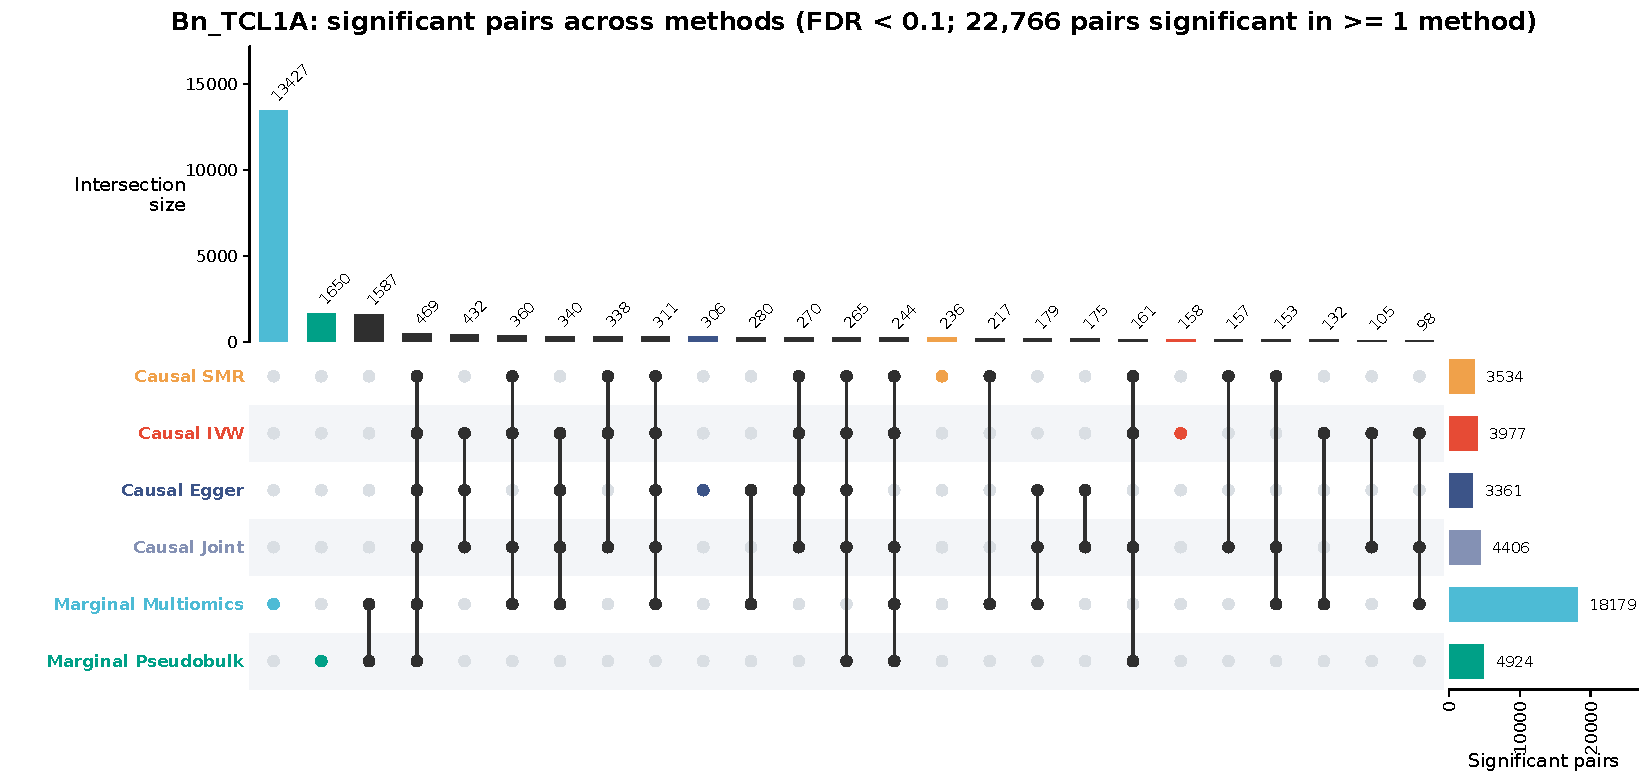
\includegraphics[page=1,width=\linewidth]{Fig1_MR_overview.pdf}\par\medskip
\includegraphics[page=4,width=\linewidth]{Fig1_MR_overview.pdf}
\caption{Overlap and direction of significant links. Top: Bn UpSet plot,
showing the 25 largest distinct significance combinations at \(\q<0.1\).
Bottom: effect-direction comparison among links significant in all six methods
in each cell type. Slices compare the IVW slope sign with the WNN and pseudobulk
correlation signs; central annotations summarize agreement among SMR, IVW,
and Egger. Existing source pages 1 and 4 are shown unchanged. The figure's
``Causal Joint'' label denotes CCT.}
\label{fig:overview}
\end{figure}

\begin{figure}[p]
\centering
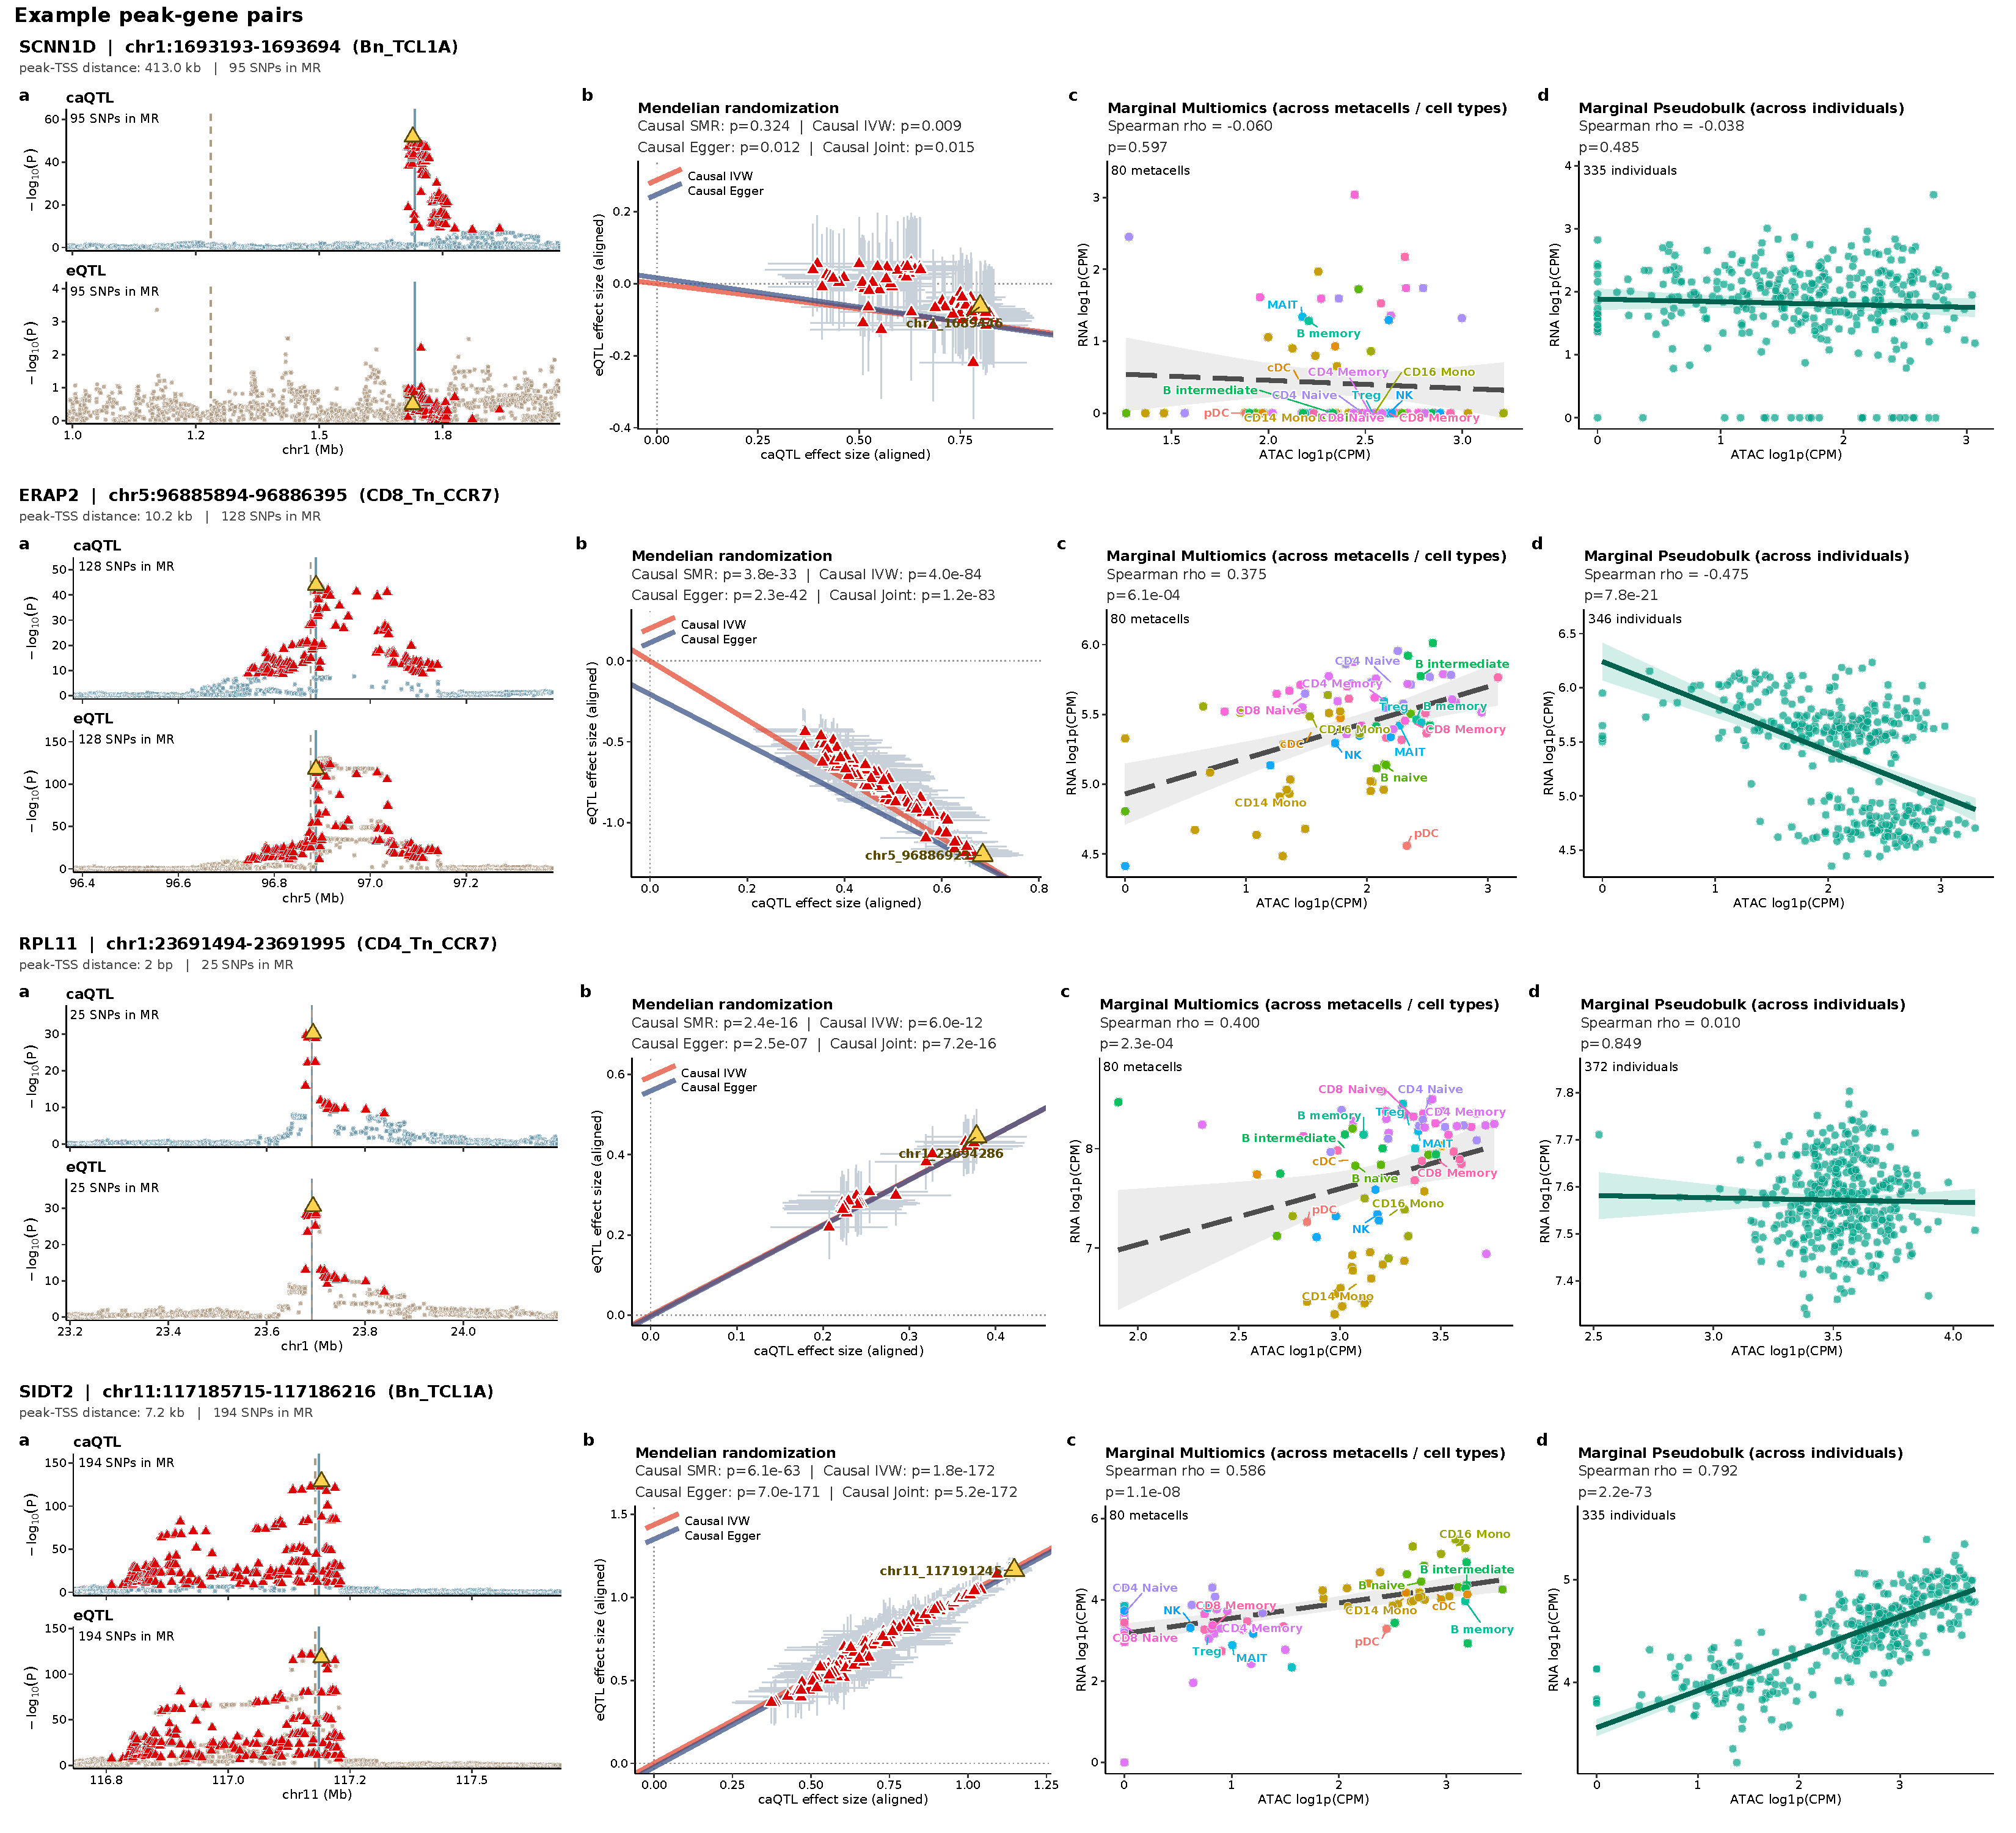
\includegraphics[page=1,width=\linewidth,height=0.79\textheight,keepaspectratio]{Fig2_examples.pdf}
\caption{Selected peak--gene examples: SCNN1D in Bn, ERAP2 in CD8, RPL11 in CD4,
and SIDT2 in Bn. Columns show QTL association tracks, aligned SNP effects with
IVW/Egger fitted lines, WNN metacell measurements, and pseudobulk measurements.
The displayed significance summaries are from the existing analysis; marginal
correlation summaries are Spearman correlations, while the drawn marginal
trend lines are linear fits. In the caQTL tracks, non-instrument variants with
\(p<10^{-8}\) are omitted by the original plotting script. Source page 1 is
shown unchanged; further examples remain in the copied six-page source PDF.
\textbf{TODO:} revise panel size and caption after example selection is reviewed.}
\label{fig:examples}
\end{figure}

\subsection{Regulatory reference support depends on the evaluation metric}
\label{res:references}
We evaluated links against EnhancerAtlas, FANTOM5, 4DGenome, GTEx, HiChIP, and
PCHiC reference datasets. The current pooled overlap summary reports enrichment
above one in every cell-type, method, and reference combination. SMR has the
largest pooled fold enrichment in 17 of 18 cell-type/reference combinations;
IVW has the largest value for CD4 PCHiC. In Bn, for example, SMR and WNN fold
enrichments are 6.18 and 3.56 against FANTOM5, and 4.46 and 3.08 against HiChIP.
The full existing summary is supplied as supporting Table~S1
(\texttt{Fig3\_Hyper\_table.xlsx}). These are descriptive comparisons of
method-specific selected sets, with different numbers of links and contributing
genes; they are not paired tests of method superiority.
% Evidence: Results/Figures/Figures_20261019/Fig3_Hyper_global.tsv.

We also summarized gene-wise ROC-AUC using raw-p-value significance scores
(Figure~\ref{fig:auc}). Differences in the stored mean AUCs were smaller and
benchmark-dependent. For Bn FANTOM5, mean AUC was 0.813 for SMR and 0.807 for
WNN, whereas for CD4 FANTOM5 it was 0.778 and 0.779, respectively. The existing
ROC calculations use automatic direction selection, so these summaries should
be read as the implemented benchmark rather than a fixed-direction ranking
comparison.
% Evidence: Results/Validation/Valid4_AUC/<CT>_AUC_long.tsv.gz.
\TODO{Select a compact reference-support table for the manuscript and develop
the interpretation of enrichment versus gene-wise discrimination.}

\begin{figure}[p]
\centering
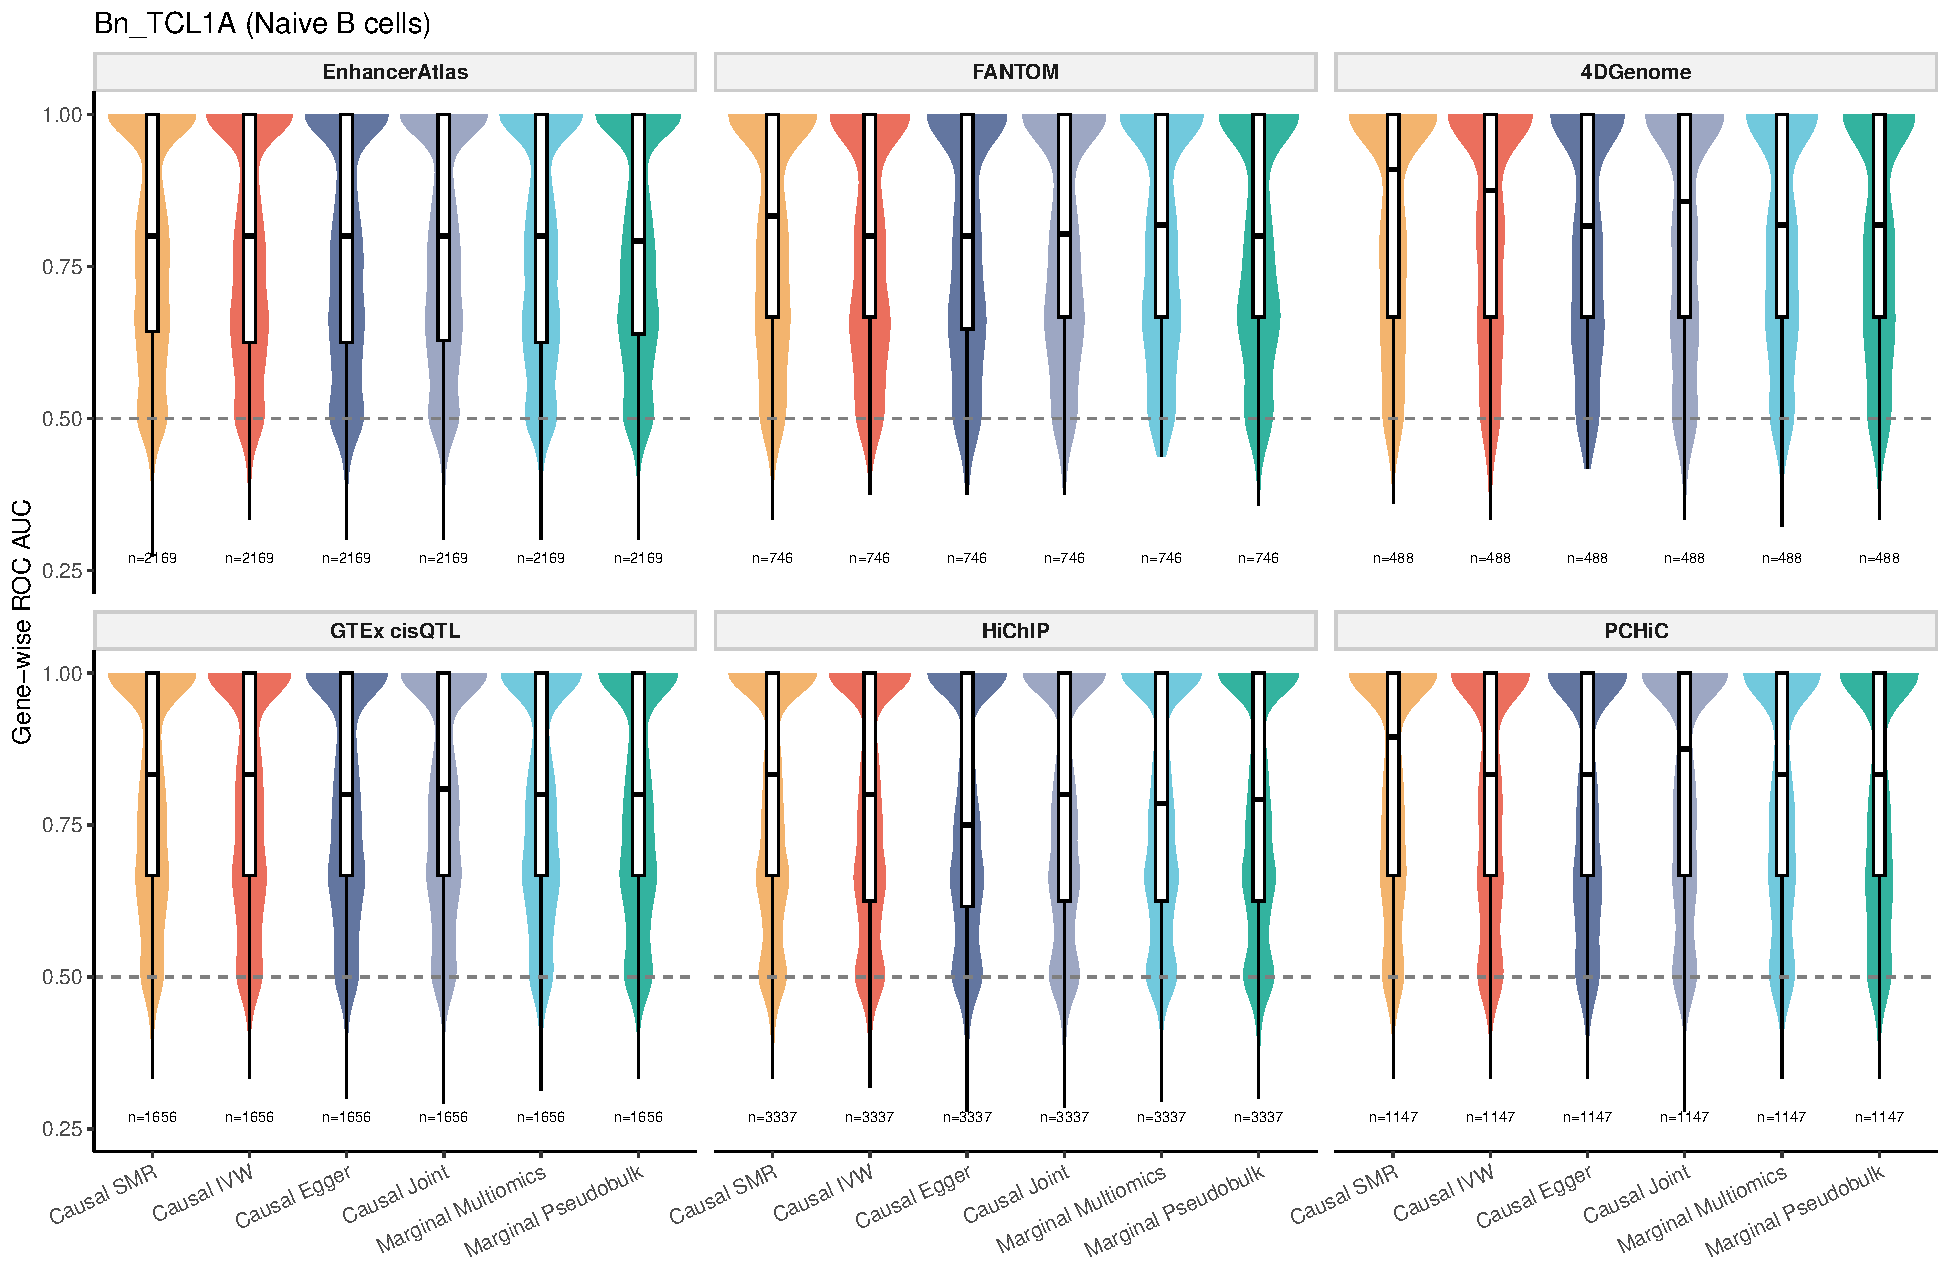
\includegraphics[page=1,width=\linewidth]{Fig4_AUC.pdf}
\caption{Gene-wise ROC-AUC against six regulatory references in Bn. Violin
and box plots summarize genes having both reference-overlapping and other
tested peaks; annotations give gene counts. Scores are \(-\log_{10}(p)\), and
ROC direction was selected automatically in the existing analysis. The dashed
line marks AUC 0.5. This is page 1 of the latest available AUC PDF, stored in
the older figure directory; CD4 and CD8 are retained as pages 2 and 3 of the
copied file.}
\label{fig:auc}
\end{figure}

\subsection{CIMA regulatory networks provide within-cohort corroboration}
\label{res:grn}
The cell-type-active CIMA SCENIC+ networks contained 864, 2,520, and 1,364
pairs from the retained Bn, CD4, and CD8 analysis sets, respectively.
At \(\q<0.05\), WNN had more network-overlapping significant pairs than SMR
(513 versus 324 in Bn), but SMR had a larger enrichment odds ratio
(9.60 versus 2.30 in Bn). This illustrates the distinction between overlap
counts and enrichment relative to the tested background
(Supplementary Figure~\ref{fig:supp-grn}). CIMA networks provide corroboration
within the same study, rather than independent experimental confirmation.
% Evidence: Valid5_GRN/GRN_summary.tsv and GRN_sig_counts_by_method.tsv.
\TODO{Integrate the high-quality eRegulon subset after deciding how much GRN
detail belongs in the main text.}

\subsection{Motifs and gene sets characterize functional relevance}
\label{res:function}
We examined motif enrichment in each method's significant peaks using
GC- and accessibility-matched backgrounds. Across 746 JASPAR motifs, the IVW
foreground yielded 58, 96, and 76 enriched motifs in Bn, CD4, and CD8,
respectively (BH-adjusted \(p<0.05\) and fold enrichment \(>1\)). The corresponding
WNN counts were 92, 123, and 92. These method-specific foregrounds are not
restricted to links unique to MR. TF-expression summaries and the existing
motif spreadsheet are supplied as supporting material (Table~S2).
% Evidence: Valid3_Motif/<CT>_motif_enrichment.tsv.gz; significance uses p.adjust.
\TODO{Choose representative TF motifs, verify their expression summaries, and
develop the biological interpretation; motif counts alone do not establish
functional specificity.}

For gene-set interpretation, we defined MR-only links as significant in at
least one of IVW, Egger, or SMR at \(\q<0.1\), with both marginal methods having
\(\q\geq0.1\). Their target genes numbered 1,581, 2,834, and 1,903, with 4,509
unique genes in the combined set. The existing GO Biological Process GSEA
returned no terms at conventional BH-adjusted \(p<0.1\) for individual cell
types, and nine for the combined set. Top combined terms include Arp2/3
complex-mediated actin nucleation and purine metabolism
(Supplementary Figure~\ref{fig:supp-go}). A separate 5,000-draw gene-set
resampling analysis returned 34, 213, 224, and 499 terms at empirical
BH-adjusted \(p<0.1\), respectively. These analyses use different null
comparisons and are kept distinct in this draft.
% Evidence: Valid7_GO/GO_GSEA_MROnly.tsv.gz; conventional p.adjust vs emp_fdr.
\TODO{Decide which GO comparison addresses the intended biological question
and select a small set of interpretable terms.}

\subsection{MR-only regions show exploratory disease-heritability enrichment}
\label{res:sldsc}
We used S-LDSC to examine peaks from MR-only links, with the definition above,
against nine immune-related GWAS. After liftOver to hg19, the MROnly sets
contained 1,271 Bn, 2,433 CD4, and 1,498 CD8 peaks; their union contained 3,777
peaks. Each extended peak annotation and the all-candidate-peak annotation
were fitted separately with baseline-LD annotations.

For the combined MROnly annotation, raw enrichment p-values were below 0.1
for Crohn's disease (CD), inflammatory bowel disease (IBD), multiple sclerosis
(MS), and type 1 diabetes (T1D), with enrichment estimates of 20.05, 18.04,
50.83, and 19.72, respectively (Figure~\ref{fig:sldsc}). Their raw p-values
ranged from 0.050 to 0.084; none met raw \(p<0.05\). These are exploratory
annotation-enrichment findings, without correction across the displayed
GWAS comparisons and without a direct test of MROnly versus all peaks.
% Evidence: Valid2_SLDSC/set_stats.tsv and SLDSC_all.tsv.
\TODO{Develop the disease interpretation and decide how to report uncertainty
alongside the existing figure, which omits standard-error bars.}

\begin{figure}[p]
\centering
\includegraphics[page=2,width=\linewidth]{Fig5_SLDSC.pdf}
\caption{S-LDSC enrichment for the union of the three cell-type MROnly peak
sets and the union of all candidate peaks. MROnly uses IVW/Egger/SMR link
\(\q<0.1\) and both marginal \(\q\geq0.1\). Peaks were lifted to hg19 and
extended by 500 bp on each side. Each custom annotation was fitted separately
with 97 baseline-LD annotations. Asterisks denote raw enrichment \(p<0.1\),
not multiplicity-adjusted significance or a test between the two bars.
AS: ankylosing spondylitis; CD: Crohn's disease; IBD: inflammatory bowel disease;
RA: rheumatoid arthritis; SLE: systemic lupus erythematosus; MS: multiple
sclerosis; T1D: type 1 diabetes; PBC: primary biliary cirrhosis, using the
source GWAS label. Source page 2 is unchanged; cell-type results are shown in
Supplementary Figure~\ref{fig:supp-sldsc}.}
\label{fig:sldsc}
\end{figure}

\subsection{GWAS-overlapping peaks nominate disease-associated regulatory examples}
\label{res:gwas}
For locus exploration, a separate, more stringent definition selected links
with any IVW, Egger, SMR, or CCT \(\q<0.001\) and both marginal \(\q\geq0.05\).
Requiring a GWAS variant with \(p<5\times10^{-8}\) inside the unextended peak
identified 27 cell-type-specific peak--gene pairs (7 Bn, 10 CD4, and 10 CD8),
covering 21 genes and 14 distinct peaks. The 37 output rows include repeated
pairs associated with different variant/trait records.

One example links the hg38 peak chr11:61827740--61828241 to TMEM258 in CD4
cells (Figure~\ref{fig:gwas}). SMR and IVW adjusted p-values were
\(2.39\times10^{-7}\) and \(8.21\times10^{-6}\), while WNN and pseudobulk
adjusted p-values were 0.398 and 0.225. The peak contains rs968567, associated
with asthma at \(p=3.67\times10^{-10}\). This positional overlap nominates a
candidate for follow-up; it does not establish colocalization or a mechanism
mediating disease risk.
% Evidence: Valid6_GWAS/GWAS_MRonly_overlap.tsv; source figure page 7.
\TODO{Review TMEM258 and alternative loci using appropriate biological
references before selecting the final disease example.}

\begin{figure}[p]
\centering
\includegraphics[page=7,width=\linewidth]{Fig8_Link_GWAS.pdf}
\caption{An asthma-associated peak linked to TMEM258 in CD4 cells. Tracks
show the gene, retained MR instruments, peak, and five method-specific links;
CCT is omitted in the original display. Solid links indicate \(\q<0.05\),
and dashed links indicate nonsignificance at that display threshold. The
purple symbol marks the overlapping GWAS variant rs968567. The x-axis is
rescaled around the peak and gene. This is unchanged source page 7 of the
27-page locus PDF; example selection remains provisional.}
\label{fig:gwas}
\end{figure}

\FloatBarrier
\section{Discussion}
\label{sec:discussion}
\textit{Preliminary outline only.}
\begin{itemize}
  \item \textbf{Principal findings.} Discuss differences in discovery yield,
  overlapping and discordant links, and the distinction between reference
  enrichment and ranking performance.
  \item \textbf{Complementary biological information.} Consider how genetic
  evidence, donor-level associations, and across-cell-type metacells address
  different aspects of regulation. Develop motif, GRN, GO, and disease-locus
  interpretations after reviewing the selected examples.
  \item \textbf{Scope of inference.} Discuss the assumptions underlying MR,
  incomplete reference labels, cell-type comparability, and the distinction
  between positional GWAS overlap and a shared causal mechanism. Present
  S-LDSC and GO exploration with their stated thresholds and null comparisons.
  \item \textbf{Limitations and future directions.} Outline source-provenance
  details still to be completed, independent validation, statistical sensitivity
  analyses if subsequently prioritized, and experimental follow-up.
\end{itemize}
\TODO{Write the Discussion after the Results narrative and figure placement
have been reviewed. Do not infer a universal advantage of MR from discovery
counts or selected examples.}

\section{Materials and Methods}
\label{sec:methods}
\textit{Structured outline; mathematical details and complete source citations
will be developed in subsequent revisions.}

\subsection{Data sources}
We used CIMA caQTL and eQTL summary statistics (OMIX009786), cell-type-specific
pseudobulk matrices, and an external PBMC multiome WNN dataset. The MR LD
reference is hg38 1000 Genomes EAS; S-LDSC uses its separate EUR reference.
\TODO{Add study citations, donor and QTL sample sizes, published covariates,
normalization, ancestry details, and data-access statements.}

\subsection{Candidate peak--gene pairs}
Precomputed cell-type-specific candidate tables supplied the pair universe.
The documented upstream search includes peaks with centers within 1 Mb of a
gene's TSS. Current eligibility requires at least three shared QTL variants
and feature availability in both marginal datasets.
\TODO{Document the definitive candidate-table generation and coordinate rules.}

\subsection{Instrument selection and LD preparation}
The model consumes pair-indexed caQTL files documented as clumped at
\(r^2=0.99\) within 20 Mb. QTL alleles must match exactly; approximately
duplicated exposure/outcome slope pairs are removed at tolerance \(10^{-3}\).
Signed PLINK LD is aligned to the retained variants, and exposure effects,
outcome effects, and LD signs are oriented together.
\TODO{Recover the original clumping command and initial instrument-selection
thresholds; give the complete retained-variant rules.}

\subsection{GLS-IVW}
IVW is fitted through the origin after whitening by the outcome-effect
covariance constructed from outcome SEs and LD. Eigenvalue truncation targets
99.9\% variance with a five-direction minimum setting, subject to available
positive directions. The implementation uses SNP-count-based degrees of
freedom and inflates SEs only for overdispersion.
\TODO{Add the GLS formulation, reference for correlated instruments, and the
precise truncation and uncertainty conventions.}

\subsection{GLS-MR Egger}
Egger uses the same LD-aware transformation and an additional intercept
\citep{bowden2015egger}. Final tables retain the slope, SE, and p-value.
\TODO{Describe the intercept and assumptions, distinguishing the general
MR-Egger reference from this project's GLS implementation.}

\subsection{Summary-data-based Mendelian randomization}
The SMR calculation uses the retained SNP with the smallest caQTL p-value,
its outcome/exposure effect ratio, and the implemented chi-square test based
on p-derived z-scores \citep{zhu2016smr}.
\TODO{Add the exact test and SE expressions. Clarify that this implementation
does not include a HEIDI analysis.}

\subsection{Cauchy combination}
CCT combines the SMR, IVW, and Egger p-values with equal weights
\citep{liu2020cauchy}. It supplies a combined significance measure rather than
a combined causal effect estimate.

\subsection{Pseudobulk and WNN correlations}
Pseudobulk Spearman correlations use matched donors and log-transformed CPM.
WNN Spearman correlations use 80 external PBMC metacells shared across the
three analyses. Neither correlation stage includes covariate residualization.
\TODO{Complete the upstream pseudobulk and metacell construction descriptions.}

\subsection{Filtering and multiple testing}
Pairs with any missing base-method p-value are removed, then pairs with IVW
residual variance greater than 10 are removed. CCT is calculated afterward.
BH adjustment is applied separately within each gene and method
\citep{benjamini1995fdr}. Discovery uses \(\q<0.1\); GRN uses \(\q<0.05\).
The two definitions of MR-only links are stated in their Results subsections.

\subsection{Regulatory references, enrichment, and ROC-AUC}
Six reference datasets are mapped to genes and genomic intervals. Gene-level
upper-tail hypergeometric tests compare significant peaks with candidate
backgrounds; the existing global summary pools eligible gene counts and reports
fold enrichment. ROC-AUC uses \(-\log_{10}(p)\), genes with both classes, and
the existing automatic ROC direction. GTEx ROC labels additionally require
overlap with validation multiome peaks.
\TODO{Add resource citations, overlap/liftOver details, reference thresholds,
and a precise definition of the comparison population.}

\subsection{Motifs, regulatory networks, and GO}
Motif analysis uses Signac, JASPAR2020, and backgrounds matched on GC and
accessibility; enrichment requires BH-adjusted \(p<0.05\) and fold \(>1\).
TF-expression checks require detection in at least 5\% of cells. GRN overlap
uses Fisher tests against all retained tested pairs. GO BP GSEA ranks MR-only
genes by minimum MR p-value over MR-only links; a separate 5,000-draw analysis
samples tested genes scored using all their links and calculates empirical
p-values from term-specific available null NES values.
\TODO{Add resource/software citations, term-size settings, gene identifiers,
and the intended interpretation of each GO null comparison.}

\subsection{Disease heritability and GWAS overlap}
S-LDSC \citep{finucane2015sldsc} evaluates hg19 peak annotations extended by
500 bp per side, each fitted with 97 baseline-LD annotations. The nine GWAS
are listed in Figure~\ref{fig:sldsc}. A separate locus screen requires a
genome-wide-significant GWAS variant inside an unextended peak.
\TODO{Add each GWAS citation and cohort description, regression resources,
uncertainty reporting, and the variant-mapping procedure.}

\subsection{Null-SNP diagnostic}
An existing diagnostic LD-prunes variants, retains caQTL/eQTL associations
with both nominal \(p>0.05\), and examines correlations of their z-scores
(Supplementary Figure~\ref{fig:supp-qc}).
\TODO{Describe its descriptive role and distinguish SNP--pair observations
from unique variants in the pooled summary.}

\FloatBarrier
\section*{Acknowledgments}
\TODO{Supply acknowledgments approved by the authors, if applicable.
Keep funding and other submission-system declarations in their dedicated
fields; see submission\_requirements.md for the outstanding information.}

\bibliography{references}
\clearpage
\section*{Supporting Information Captions}
% Supporting graphics remain visible in this drafting version.
\setcounter{figure}{0}
\renewcommand{\thefigure}{S\arabic{figure}}
\renewcommand{\theHfigure}{supp.\arabic{figure}}
\captionsetup[figure]{labelformat=plossupport}

Supporting Table~S1 is the copied regulatory-enrichment workbook
\path{figures/Fig3_Hyper_table.xlsx}. Supporting Table~S2 is the copied
motif workbook \path{figures/Fig6_Motif_table.xlsx}. They remain native
spreadsheets and are not rendered as LaTeX figures. Table~S2 has updated numeric
cells but inherited manual biological annotations; its ``MR-only'' title
should be reviewed because the underlying foregrounds are method-specific.
\TODO{Convert selected supporting-table content to manuscript tables after
review; do not treat inherited annotation text as independently verified.}

\noindent\textbf{S1 Table. Regulatory-reference enrichment workbook.}
\TODO{Finalize the supporting-table caption and file format after review of
the existing workbook; no table content has been revised.}

\noindent\textbf{S2 Table. Motif enrichment workbook.}
\TODO{Finalize the supporting-table caption after review of the inherited
annotations and foreground description noted above.}

\noindent\textbf{S1 Checklist. STROBE-MR reporting checklist (pending).}
\TODO{Prepare the completed reporting checklist with manuscript page numbers
and relevant text. This label reserves a supporting item; no completed
checklist is currently supplied.}

\begin{figure}[p]
\centering
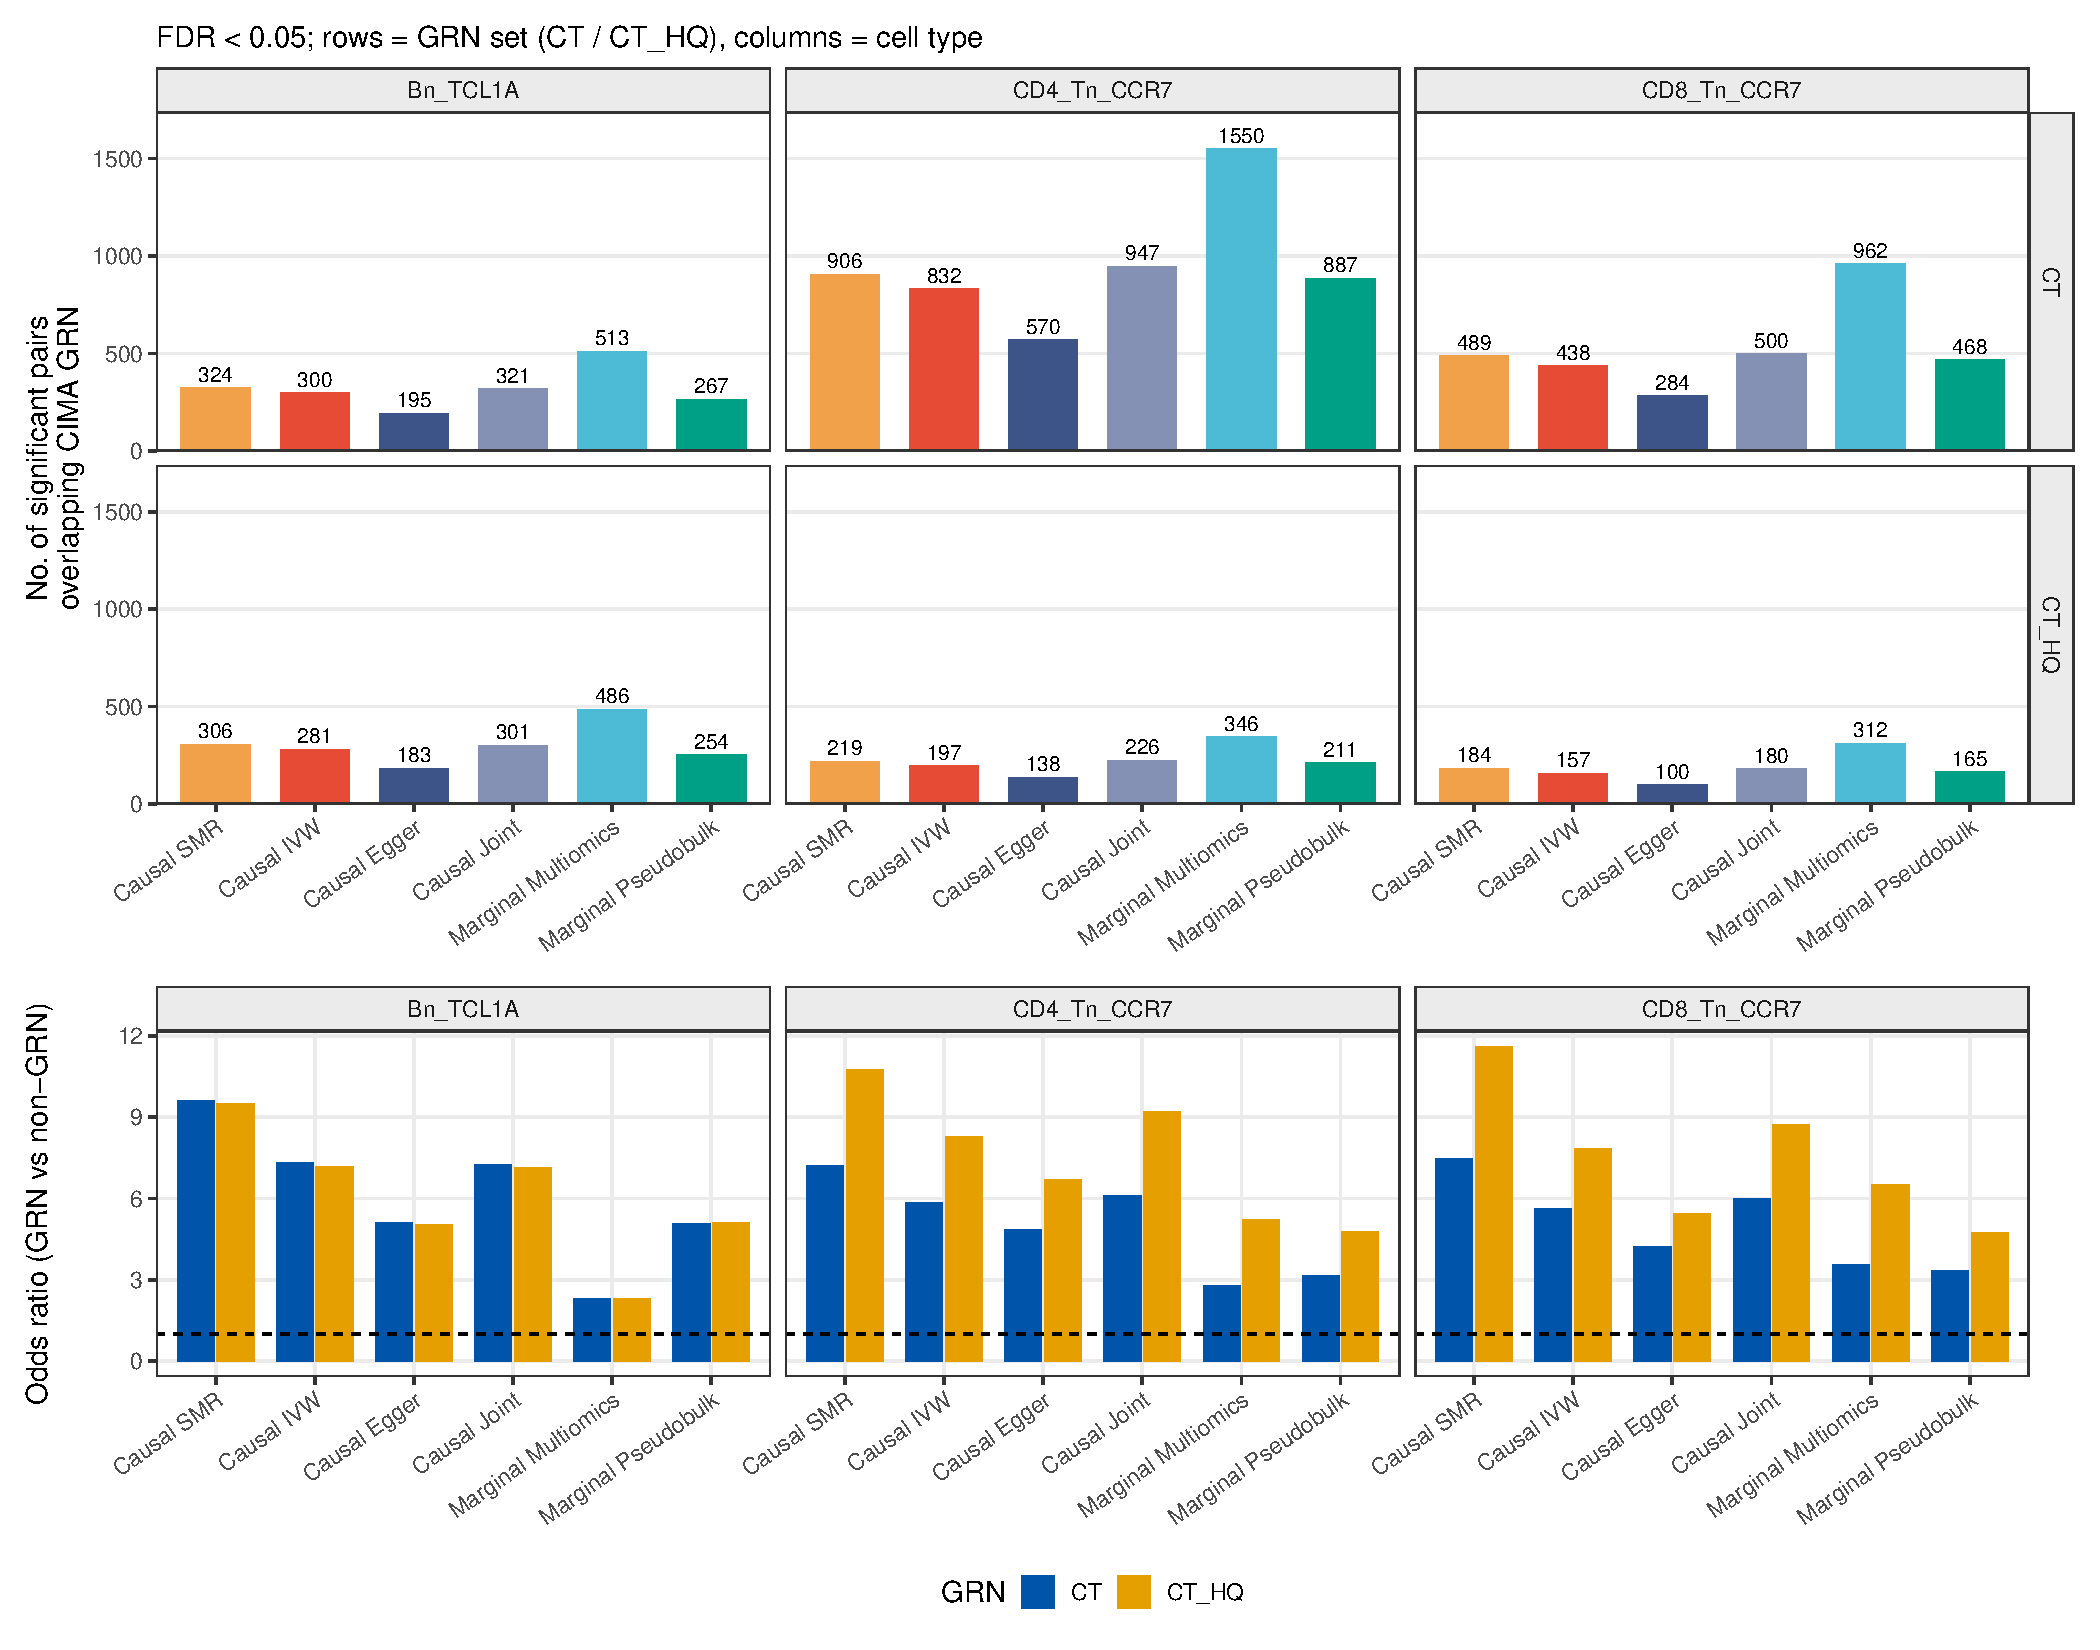
\includegraphics[page=1,width=\linewidth,height=0.78\textheight,keepaspectratio]{Fig7_GRN.pdf}
\caption{Within-CIMA GRN corroboration. Top panels show significant-pair
overlap counts at \(\q<0.05\) for cell-type-active networks (CT) and their
lineage high-quality subset (CT\_HQ). Bottom panels show Fisher odds ratios
relative to non-GRN tested pairs. This unchanged one-page figure is the latest
available GRN artifact in the older figure directory.}
\label{fig:supp-grn}
\end{figure}

\begin{figure}[p]
\centering
\includegraphics[page=2,width=\linewidth,height=0.70\textheight,keepaspectratio]{Fig9_GO_GSEA.pdf}
\caption{Conventional GO BP GSEA for the 4,509 combined MR-only target genes.
The five terms with smallest conventional GSEA p-values are shown as
\(-\log_{10}\) BH-adjusted p-values; the dashed line marks adjusted \(p=0.1\).
This is unchanged source page 2. Pages 1 and 3 of the copied PDF contain
per-group conventional-p and empirical-p displays, respectively, and are not
silently combined with this conventional comparison.}
\label{fig:supp-go}
\end{figure}

\begin{figure}[p]
\centering
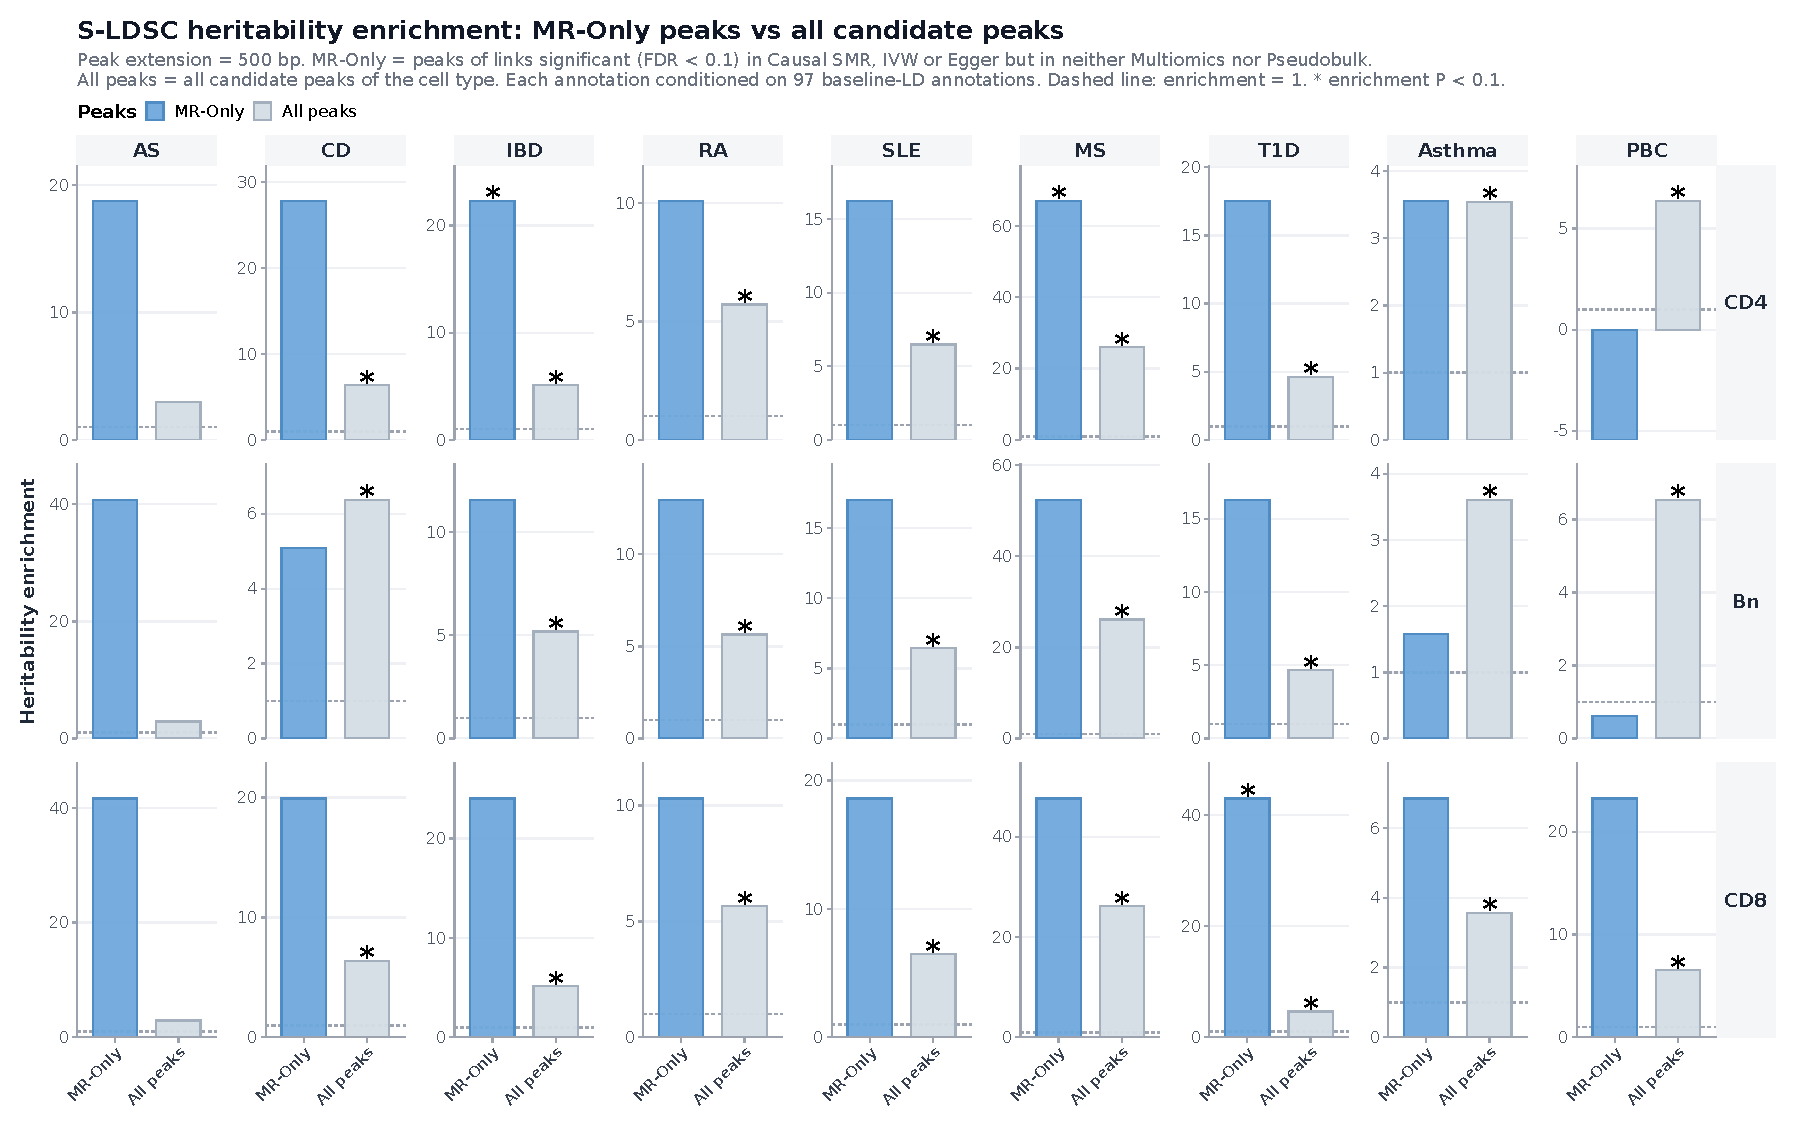
\includegraphics[page=1,width=\linewidth]{Fig5_SLDSC.pdf}
\caption{Cell-type-specific S-LDSC enrichment. The unchanged source page 1
compares MROnly and all-candidate-peak annotations for CD4, Bn, and CD8, with
the definition and raw-p asterisk convention of Figure~\ref{fig:sldsc}.
Axis scales differ between panels.}
\label{fig:supp-sldsc}
\end{figure}

\begin{figure}[p]
\centering
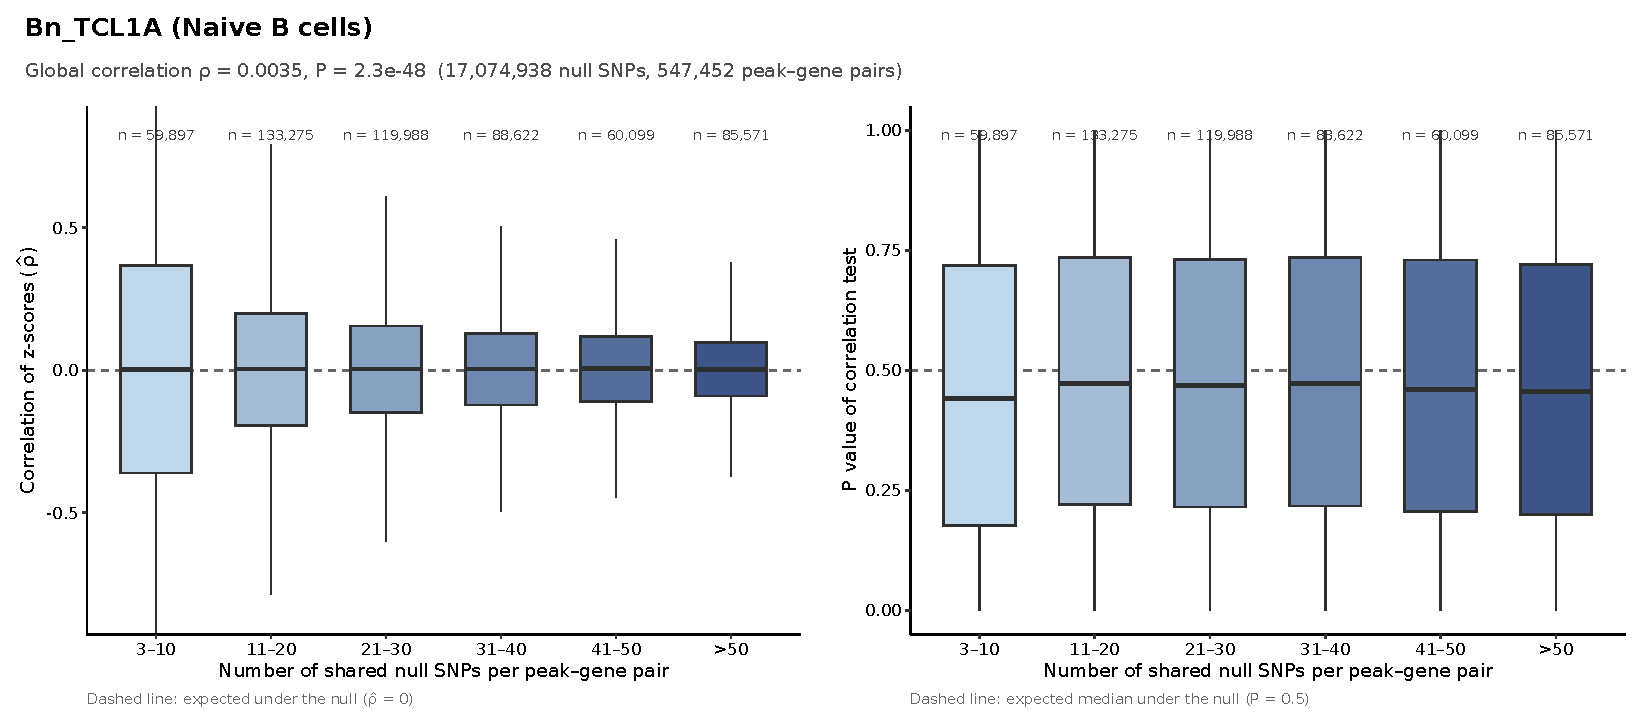
\includegraphics[page=1,width=\linewidth]{Sup1_OneSampleMR.pdf}
\caption{Null-SNP diagnostic in Bn. Pair-level correlations of caQTL and
eQTL z-scores, and their correlation-test p-values, are grouped by the number
of shared pruned null SNPs. The displayed global summary pools SNP--pair
observations; repeated variants may contribute to multiple pairs. This is
unchanged source page 1, with CD4 and CD8 retained as pages 2 and 3 in the
copied PDF. The diagnostic does not itself establish MR calibration.}
\label{fig:supp-qc}
\end{figure}
\FloatBarrier

\end{document}
